\documentclass[10pt,twocolumn]{article}
\usepackage[a4paper,margin=0.8in,columnsep=0.28in]{geometry}
\usepackage[T1]{fontenc}
\usepackage{mathptmx}
\usepackage[utf8]{inputenc}
\usepackage{microtype}
\usepackage{amsmath,amssymb}
\usepackage{booktabs}
\usepackage{multirow}
\usepackage{graphicx}
\usepackage{xcolor}
\usepackage[labelfont=bf,font=small,labelsep=period]{caption}
\usepackage{enumitem}
\usepackage[numbers,sort&compress]{natbib}
\usepackage[hidelinks]{hyperref}
\setlist{nosep,leftmargin=1.3em}
\setlength{\parskip}{0pt}
\setlength{\bibsep}{1pt}
\renewcommand{\bibfont}{\small}
\newcommand{\revision}{\texttt{submission}}
\newcommand{\todo}[1]{\textcolor{red}{#1}}
\newcommand{\Chr}{Chronos-2}

\title{\vspace{-0.4em}\textbf{Reliable Probabilistic Time Series Imputation:\\ When Are Predictive Distributions Trustworthy?}\vspace{-0.3em}}
\author{Vladislav Voronin \quad Kirill Lalayants \quad Mikhail Bezrukov \quad Fedor Zhirkov\\[2pt]
\small Course project, Models of Sequential Data \quad Supervisor: Vitaliy Pozdnyakov}
\date{\vspace{-1.2em}}

\begin{document}
\maketitle

\begin{abstract}
\noindent
Imputation methods are usually scored on how close the median is to the missing value. Many uses need a predictive distribution, and then the question is whether its intervals can be trusted. We compare three imputers on three real datasets (ETT\_h1, Electricity, BeijingAir PM2.5): a local-level Kalman smoother, CSDI (a conditional diffusion model), and the frozen forecasting model \Chr{} used from both sides of a gap by averaging a forward and a time-reversed forecast. All models see the same saved masks (24 or 128 hidden values, scattered or as one block) and are scored with pinball loss, CRPS, and calibration errors, with paired cluster-bootstrap intervals. Contiguous blocks are harder than scattered points for every model. CSDI trained for 100 epochs is best or tied with the best in all 12 test cells, but a 40-epoch CSDI was clearly under-trained, and with it the ranking looked different. No model has well-calibrated 80\% intervals: CSDI covers 0.71--0.75, the Kalman smoother covers 0.71--0.95, and the \Chr{} blend covers 0.67--0.90. On synthetic local-level data with an exact reference, averaging quantiles gives intervals 11--24\% wider than the exact ones, and a Gaussian product of the two forecasts is 13--28\% too narrow with coverage 0.56--0.67. A time-reversal test shows an effect on an irreversible synthetic process and none on a reversible one; on the real data we see no consistent direction. We report the negative results and the limits of the evidence, including a single CSDI seed and an unchecked pretraining overlap for \Chr{}.
\end{abstract}

\section{Introduction}
A time series with gaps is a common input: sensors fail, meters are offline, stations stop reporting. Imputation fills the gaps, and most benchmarks judge it by the error of a single filled value \citep{du2024tsibench}. When the filled series feeds a decision, the width of the uncertainty matters as much as the value. A model that reports an 80\% interval is useful only if about 80\% of the hidden values fall inside it.

We ask: \emph{when are native predictive distributions of imputers reliable, and how does a two-sided forecasting adaptation affect calibration?} Three hypotheses guide the study.
\begin{description}[leftmargin=0pt,labelindent=0pt,itemsep=1pt]
\item[H1] Contiguous blocks are harder than scattered points at the same number of hidden values.
\item[H2] Median accuracy and calibration can disagree.
\item[H3] Blending a left-side and a right-side forecast can change calibration, in either direction.
\end{description}

\paragraph{Contributions.}
\begin{enumerate}
\item A protocol that gives a classical smoother, a diffusion model and a pretrained forecaster the same windows, masks and metrics (Sections~\ref{sec:setup}--\ref{sec:eval}).
\item A comparison on 12 test cells (3 datasets $\times$ 4 mask settings) with paired cluster-bootstrap intervals, so that ties are reported as ties (Section~\ref{sec:results}).
\item A synthetic test with an exact reference that measures how much the quantile blend widens the intervals, and a time-reversal test of the two-sided adaptation (Sections~\ref{sec:blend}, \ref{sec:reversal}).
\item An account of failures: an under-trained CSDI, a discarded training run, and variants that did not help (Section~\ref{sec:limits}).
\end{enumerate}

\section{Related Work}
\textbf{Imputation benchmarks.} TSI-Bench \citep{du2024tsibench} and the PyPOTS toolbox \citep{du2023pypots} compare many imputers on point error. We use PyPOTS for CSDI. Our setting differs by scoring distributions and by a shared mask file for all models. \textbf{Diffusion imputation.} CSDI \citep{tashiro2021csdi} trains a conditional score-based diffusion model on observed and masked entries and samples the missing ones. \textbf{Foundation models.} Chronos \citep{ansari2024chronos} and Chronos-2 \citep{ansari2025chronos2} are pretrained forecasters that output quantiles. Their calibration is studied for forecasting by \citet{adler2026beyond}; we ask the same question for imputation, where a forecast has to be adapted to a gap with context on both sides. \textbf{Scoring and evaluation.} Pinball loss and CRPS are proper scores \citep{koenker1978,gneiting2007}; our calibration errors follow the idea of quantile calibration \citep{kuleshov2018}. Forecast-evaluation practice, including dependence between test cases and the risk of reading small differences as findings, is discussed by \citet{bergmeir2023}. This motivates our paired intervals. The local-level Kalman smoother is textbook state-space material \citep{kalman1960,durbin2012}.

\section{Problem Setup and Data}\label{sec:setup}
\textbf{Task.} A window of 256 consecutive values of one channel has $k\in\{24,128\}$ hidden values. The model sees the rest and returns, for each hidden position, a predictive distribution (quantiles, or samples that we turn into quantiles). Only hidden positions are scored. The first and last 24 positions of a window always stay observed.

\textbf{Masks.} Two patterns with the same hidden count: \emph{point} (scattered positions) and \emph{block} (one contiguous gap). Together with $k$ this gives four mask settings. All four use the same windows. Masks are saved to disk and read by every model. Validation and test use different seeds (1 and 2).

\begin{table}[t]
\centering\small
\setlength{\tabcolsep}{4pt}
\begin{tabular}{@{}lrrrl@{}}
\toprule
Dataset & Chan. & Steps & Test ch. & Notes \\
\midrule
ETT\_h1 & 7 & 17,420 & 7 & transformer temp.\\
Electricity & 20 & 26,305 & 19 & hourly means\\
BeijingAir & 12 & 35,064 & 12 & PM2.5, 2.08\% gaps\\
\bottomrule
\end{tabular}
\caption{Datasets. ``Test ch.'' counts channels that contributed at least one test window.}
\label{tab:data}
\end{table}

\textbf{Data.} ETT\_h1 \citep{zhou2021informer} has 7 channels. Electricity \citep{trindade2015} uses the first 20 clients by id that have no zero run longer than 24 hours in the training part, starting in 2012 (earlier years have long zero runs), aggregated to hourly means. BeijingAir \citep{zhang2017} is PM2.5 at 12 stations, one univariate channel each. Table~\ref{tab:data} gives sizes.

\textbf{Split and windows.} Each dataset is split chronologically 60/20/20 into train, validation and test. Scaling statistics (mean and standard deviation per channel), Kalman variances and CSDI weights use the train part only. Every window lies fully inside one split and has no native missing value. We draw 60 windows per dataset and split, across channels. In the test split ETT\_h1 contributes 6 to 10 windows per channel, Electricity 1 to 6, and BeijingAir comes from 12 stations. The number of eligible windows per dataset was not recorded, which we list as a limitation. All errors are in train-scaled units, except MRE which uses the original scale.

\textbf{Leakage.} The three models can use only observed values of the window and train-split statistics. The \Chr{} model is pretrained on external data. We did not check whether any of our three datasets, or the periods used for testing, occur in its pretraining corpus; we did not resolve this against the corpora named in the \Chr{} paper. If there is overlap, the \Chr{} results are optimistic.

\section{Methods}\label{sec:methods}
\textbf{Kalman smoother (classical baseline).} A local-level model $x_t=x_{t-1}+\eta_t$, $y_t=x_t+\varepsilon_t$ with process variance $q$ and observation variance $r$ fitted per channel by maximum likelihood on the last 6,000 train points. The predictive distribution of a hidden measurement is Gaussian with the smoothed state variance plus $r$. Parameter uncertainty is not included. The model has no seasonality and no cross-channel input.

\textbf{CSDI (diffusion model).} We use the PyPOTS implementation with one model per dataset, trained on univariate windows pooled over channels: 413,521 parameters, 4 layers, 8 heads, 50 diffusion steps, 6,000 training windows, 200 validation windows, batch size 32. Training masks come half from our point and block masks (1 to 128 hidden values) and half from the PyPOTS random-ratio strategy. At test time we draw 100 samples per window and read quantiles from them. Two training budgets are reported.
\begin{itemize}
\item \textbf{CSDI-40}: PyPOTS default (Adam, constant learning rate $10^{-3}$), at most 40 epochs, early stopping on validation loss with patience 5. This was our first run.
\item \textbf{CSDI-100}: Adam with learning rate $10^{-3}$ divided by 10 at 75\% and 90\% of the optimizer steps (steps 14,100 and 16,920 of 18,800), 100 epochs, no early stopping, the same windows, PyTorch seed 0. The original CSDI recipe uses 200 epochs and batch size 16; we use 100 and 32.
\end{itemize}
CSDI-100 is our main CSDI. It was added after the peer review of the first results, which asked whether CSDI had trained enough. We fixed the recipe once and ran it on all three datasets. Validation loss only chooses the saved epoch.

\textbf{\Chr{} (frozen forecaster).} We use \texttt{chronos-2-small} without fine-tuning. For each run of $k$ hidden values we forecast the run from the left prefix, and from the reversed right suffix (forecasting the reversed series and flipping it back). Other hidden runs stay as missing values in the context. The two forecasts give quantile functions $Q^{L}_j(\tau)$ and $Q^{R}_j(\tau)$ at position $j=1,\dots,k$ of the run. The blend averages matching quantiles with linear weights
\begin{equation}
Q_j(\tau)=w_j\,Q^{L}_j(\tau)+(1-w_j)\,Q^{R}_j(\tau),\quad w_j=\tfrac{k-j}{k+1}.
\end{equation}
Positions near the left edge lean on the left forecast, and positions near the right edge on the right forecast. This is a heuristic. It is not the distribution conditional on both sides. We also test two variants: equal weights ($w_j=\tfrac12$) and a Gaussian product of experts (PoE), where each forecast is turned into a normal distribution (median, and scale from the 0.1 and 0.9 quantiles), and the two normals are multiplied (precision-weighted mean, summed precisions).

\section{Evaluation}\label{sec:eval}
\textbf{Accuracy.} MAE, MSE, RMSE, MRE of the median. \textbf{Probabilistic.} Pinball loss averaged over nine levels $\tau=0.1,\dots,0.9$ is the common score for all models. CRPS has a different estimate per family (analytic for Kalman, from samples for CSDI, twice the mean pinball over the saved levels for \Chr{}). To compare on equal footing we also compute CRPS$_{21}$, the quantile approximation on one 21-level grid for all models. NLL exists only for Kalman.

\textbf{Calibration.} PCE is the mean gap between nominal level $\tau$ and the observed frequency of $y\le Q(\tau)$. CCE is the mean of $s-\mathrm{coverage}(s)$ over central intervals $s\in\{0.2,0.4,0.6,0.8,0.9\}$: positive values mean undercoverage, negative values mean overcoverage. We also report 80\% coverage and width, and SIW (width divided by the spread of the targets). Width and coverage are read together, because wide intervals cover more without being better calibrated.

\textbf{Uncertainty of differences.} Windows from the same channel are dependent, and channels differ a lot. We resample channels, then windows within the sampled channels, 2,000 times, keeping all models on the same window together. The 95\% interval of the paired difference gives a verdict; if it contains zero, the models are \emph{tied}. Only 7 to 19 channels exist per dataset, so the intervals are rough, and we apply no multiple-comparison correction.

\textbf{Synthetic checks.} (i) \emph{Oracle test.} Local-level series ($q=1$, $r/q\in\{0.01,0.1,1\}$), 1,000 windows of 256 steps, one block of 24 or 128 hidden values. The exact Kalman smoother with the true parameters gives the reference distribution. (ii) \emph{Time reversal.} A reversible AR(1) process ($\phi=0.9$) and an irreversible jump process (jumps with probability 0.03 and exponential size, decay 0.9). The left and right forecasts are compared with the full context and with equal context lengths on both sides.

\begin{table*}[t]
\centering\small
\setlength{\tabcolsep}{5pt}
\begin{tabular}{@{}l cccc c cccc@{}}
\toprule
 & \multicolumn{4}{c}{Pinball (nine levels)} & & \multicolumn{4}{c}{MAE of the median}\\
\cmidrule(lr){2-5}\cmidrule(l){7-10}
Cell & Kalman & CSDI-40 & \Chr{} blend & CSDI-100 & & Kalman & CSDI-40 & \Chr{} blend & CSDI-100\\
\midrule
ETT\_h1 point 24 & 0.0882 & 0.0888 & 0.0832 & \textbf{0.0755} &  & 0.2102 & 0.2254 & 0.2093 & \textbf{0.1899} \\
ETT\_h1 block 24 & 0.3520 & 0.1594 & \textbf{0.1282} & 0.1302$^\dagger$ &  & 0.8625 & 0.4006 & \textbf{0.3299} & 0.3321 \\
ETT\_h1 point 128 & 0.1275 & 0.1152 & 0.1077 & \textbf{0.0895} &  & 0.3142 & 0.2910 & 0.2711 & \textbf{0.2258} \\
ETT\_h1 block 128 & 0.3404 & 0.2560 & 0.1711$^\dagger$ & \textbf{0.1605} &  & 0.7981 & 0.6335 & 0.4244 & \textbf{0.4099} \\
\midrule
Electricity point 24 & 0.0841 & 0.0705 & 0.0710 & \textbf{0.0578} &  & 0.2012 & 0.1790 & 0.1782 & \textbf{0.1469} \\
Electricity block 24 & 0.2678 & 0.1142$^\dagger$ & 0.1118$^\dagger$ & \textbf{0.1055} &  & 0.6627 & 0.2885 & 0.2830 & \textbf{0.2655} \\
Electricity point 128 & 0.1363 & 0.0869 & 0.0968 & \textbf{0.0734} &  & 0.3369 & 0.2204 & 0.2425 & \textbf{0.1874} \\
Electricity block 128 & 0.3449 & 0.1463 & 0.1580$^\dagger$ & \textbf{0.1300} &  & 0.7225 & 0.3635 & 0.3927 & \textbf{0.3222} \\
\midrule
BeijingAir point 24 & 0.0450 & 0.0444 & 0.0495 & \textbf{0.0382} &  & \textbf{0.0942} & 0.1118 & 0.1140 & 0.0954 \\
BeijingAir block 24 & 0.1599$^\dagger$ & 0.1809 & 0.1612$^\dagger$ & \textbf{0.1482} &  & \textbf{0.3789} & 0.4563 & 0.4224 & 0.3810 \\
BeijingAir point 128 & 0.0677 & 0.0643 & 0.0831 & \textbf{0.0590} &  & 0.1480 & 0.1605 & 0.2037 & \textbf{0.1462} \\
BeijingAir block 128 & 0.3513 & 0.3387 & 0.3363 & \textbf{0.2968} &  & 0.8491 & 0.8551 & 0.8348 & \textbf{0.7407} \\
\bottomrule

\end{tabular}
\caption{Test results per cell (60 windows). Bold: lowest mean. $^\dagger$: tied with the best on pinball (95\% interval of the paired difference contains zero). The cells are dataset, mask pattern, hidden count.}
\label{tab:main}
\end{table*}

\section{Results}\label{sec:results}
\subsection{Accuracy and ranking}
Table~\ref{tab:main} gives every cell. Averaged over the 12 cells, pinball is 0.197 for Kalman, 0.139 for CSDI-40, 0.130 for the \Chr{} blend and 0.114 for CSDI-100 (Table~\ref{tab:summary}). CSDI-100 has the lowest mean in 11 cells; in the twelfth (ETT\_h1 block 24) the blend is best and the two are tied.

Table~\ref{tab:pairs} counts verdicts of the paired intervals over the 12 cells. CSDI-100 beats the blend in all six point cells and ties with it in five of six block cells. It never loses significantly to Kalman or to the blend, and it improves on CSDI-40 in 11 cells (one tie). The ranking of CSDI depends on its training budget: with CSDI-40 the blend wins 4 cells, ties 5 and loses 3. The first picture, ``CSDI and the blend are comparable'', becomes ``CSDI-100 is at least as good as the blend'' after 60 more epochs with a decaying learning rate.

The Kalman smoother comes closest to the learned models on scattered gaps in BeijingAir (point 24: 0.0450, against 0.0444 for CSDI-40 and 0.0382 for CSDI-100) and is weak on blocks in ETT\_h1 and Electricity (ETT\_h1 block 24: 0.352 against 0.130 for the blend). A local-level model has no daily cycle, which may explain the block results on load and temperature data; we did not test this with a seasonal state-space model.

\textbf{H1 holds.} At equal hidden counts, blocks have higher MAE and CRPS than scattered points for every model in all six dataset$\times$hidden-count comparisons (Table~\ref{tab:h1}). The block to point ratio is between 1.5 and 5.7. Pinball shows the same.

\begin{table}[t]
\centering\small
\setlength{\tabcolsep}{3.5pt}
\begin{tabular}{@{}lcccc@{}}
\toprule
 & \multicolumn{2}{c}{MAE} & \multicolumn{2}{c}{CRPS}\\
\cmidrule(lr){2-3}\cmidrule(l){4-5}
Model & cells & ratio & cells & ratio\\
\midrule
Kalman & 6/6 & 2.14--5.74 & 6/6 & 2.54--5.15 \\
CSDI-40 & 6/6 & 1.61--5.33 & 6/6 & 1.62--5.27 \\
CSDI-100 & 6/6 & 1.72--5.07 & 6/6 & 1.73--5.03 \\
Chronos blend & 6/6 & 1.57--4.10 & 6/6 & 1.53--4.03 \\
\bottomrule

\end{tabular}
\caption{H1: block against point at equal hidden count. ``cells'': number of the 6 dataset$\times$hidden-count pairs where block is worse than point. ``ratio'': range of block/point.}
\label{tab:h1}
\end{table}

\begin{table}[t]
\centering\small
\setlength{\tabcolsep}{3pt}
\begin{tabular}{@{}lccc cc@{}}
\toprule
 & \multicolumn{3}{c}{All 12 cells} & Point & Block\\
Pair (first vs second) & 1st & tie & 2nd & \multicolumn{2}{c}{1st/tie/2nd}\\
\midrule
CSDI-100 vs Chronos blend & 7 & 5 & 0 & 6/0/0 & 1/5/0 \\
CSDI-100 vs Kalman & 11 & 1 & 0 & 6/0/0 & 5/1/0 \\
CSDI-100 vs CSDI-40 & 11 & 1 & 0 & 6/0/0 & 5/1/0 \\
CSDI-40 vs Kalman & 8 & 4 & 0 & 4/2/0 & 4/2/0 \\
Chronos blend vs Kalman & 7 & 3 & 2 & 3/1/2 & 4/2/0 \\
Chronos blend vs CSDI-40 & 4 & 5 & 3 & 1/2/3 & 3/3/0 \\
Chronos blend vs Chronos left & 11 & 1 & 0 & 6/0/0 & 5/1/0 \\
Chronos blend vs Chronos right & 11 & 1 & 0 & 6/0/0 & 5/1/0 \\
\bottomrule

\end{tabular}
\caption{Paired cluster-bootstrap verdicts on pinball. ``1st'' counts cells where the first model has the lower loss with the interval excluding zero.}
\label{tab:pairs}
\end{table}

\begin{table*}[t]
\centering\small
\setlength{\tabcolsep}{6pt}
\begin{tabular}{@{}lcccccccc@{}}
\toprule
Model & MAE & Pinball & CRPS$_{21}$ & PCE & CCE & Cov.\ 80\% & Width 80\% & SIW\\
\midrule
Kalman & 0.465 & 0.197 & 0.349 & 0.057 & $-$0.101 & 0.850 & 1.819 & 0.777 \\
CSDI-40 & 0.349 & 0.139 & 0.246 & 0.064 & 0.072 & 0.704 & 0.876 & 0.359 \\
CSDI-100 & 0.287 & 0.114 & 0.201 & 0.027 & 0.047 & 0.733 & 0.792 & 0.326 \\
Chronos left & 0.395 & 0.158 & 0.279 & 0.025 & 0.015 & 0.775 & 1.211 & 0.489 \\
Chronos right & 0.391 & 0.157 & 0.279 & 0.029 & 0.014 & 0.777 & 1.190 & 0.483 \\
Chronos blend & 0.326 & 0.130 & 0.230 & 0.034 & $-$0.033 & 0.831 & 1.115 & 0.452 \\
\bottomrule

\end{tabular}
\caption{Test means over the 12 cells. Nominal 80\% coverage is 0.80. CCE is positive for undercoverage and negative for overcoverage. Averaging over cells hides the range inside each model; Table~\ref{tab:calib} in the appendix lists every cell.}
\label{tab:summary}
\end{table*}

\subsection{Calibration}
Table~\ref{tab:summary} shows that the three models miss the nominal level in different ways.

\textbf{CSDI undercovers.} CSDI-40 covers 0.70 on average (CCE $+0.072$). Longer training moves the numbers in the right direction without fixing them. PCE falls from 0.064 to 0.027, falls in all 12 cells, and CSDI-100 has the lowest PCE of the four main models in 9 cells. The 80\% intervals get narrower in 11 of 12 cells, and coverage stays between 0.710 and 0.750. CCE is positive in all 12 cells. The bootstrap interval of the 80\% coverage contains 0.80 in only one cell (ETT\_h1 block 24; for CSDI-40 in none). CSDI-100 gives sharper and more accurate intervals that are still too narrow.

\textbf{Kalman overcovers on average, with a wide range.} Its mean coverage is 0.85 and the range over cells is 0.71 to 0.95. It has the widest intervals (mean 1.82 against 0.79 for CSDI-100). Figure~\ref{fig:along} in the appendix shows its width growing as an arc with the distance from the edges of a gap. The reliability curves in Figure~\ref{fig:reliability} show it too wide on long blocks: on Electricity block 128 its observed frequency rises from about 0.07 at $\tau=0.2$ to about 0.77 at $\tau=0.6$.

\textbf{The \Chr{} blend is close to nominal or above it.} Mean coverage is 0.83 (range 0.67 to 0.90), and 9 of 12 cells are above 0.80. It undercovers on long BeijingAir gaps (0.67 for block 128).

\textbf{Pooled numbers hide channel differences.} Per channel, the share of channels whose 80\% coverage is more than 0.10 away from 0.80 (average over cells) is 0.26 for the blend, 0.47 for CSDI-40 and 0.49 for Kalman. We did not compute this for CSDI-100.

\textbf{H2: accuracy and calibration disagree.} Among the four main models, the lowest-MAE model differs from the lowest-PCE model in 5 of 12 cells. Across all six rows of Table~\ref{tab:summary}, the lowest mean PCE belongs to the left-only \Chr{} forecast (0.025), which is clearly less accurate than CSDI-100 (pinball 0.158 against 0.114). Low calibration error therefore does not identify the better imputer, and a better imputer does not have to be calibrated.

\begin{figure*}[t]
\centering
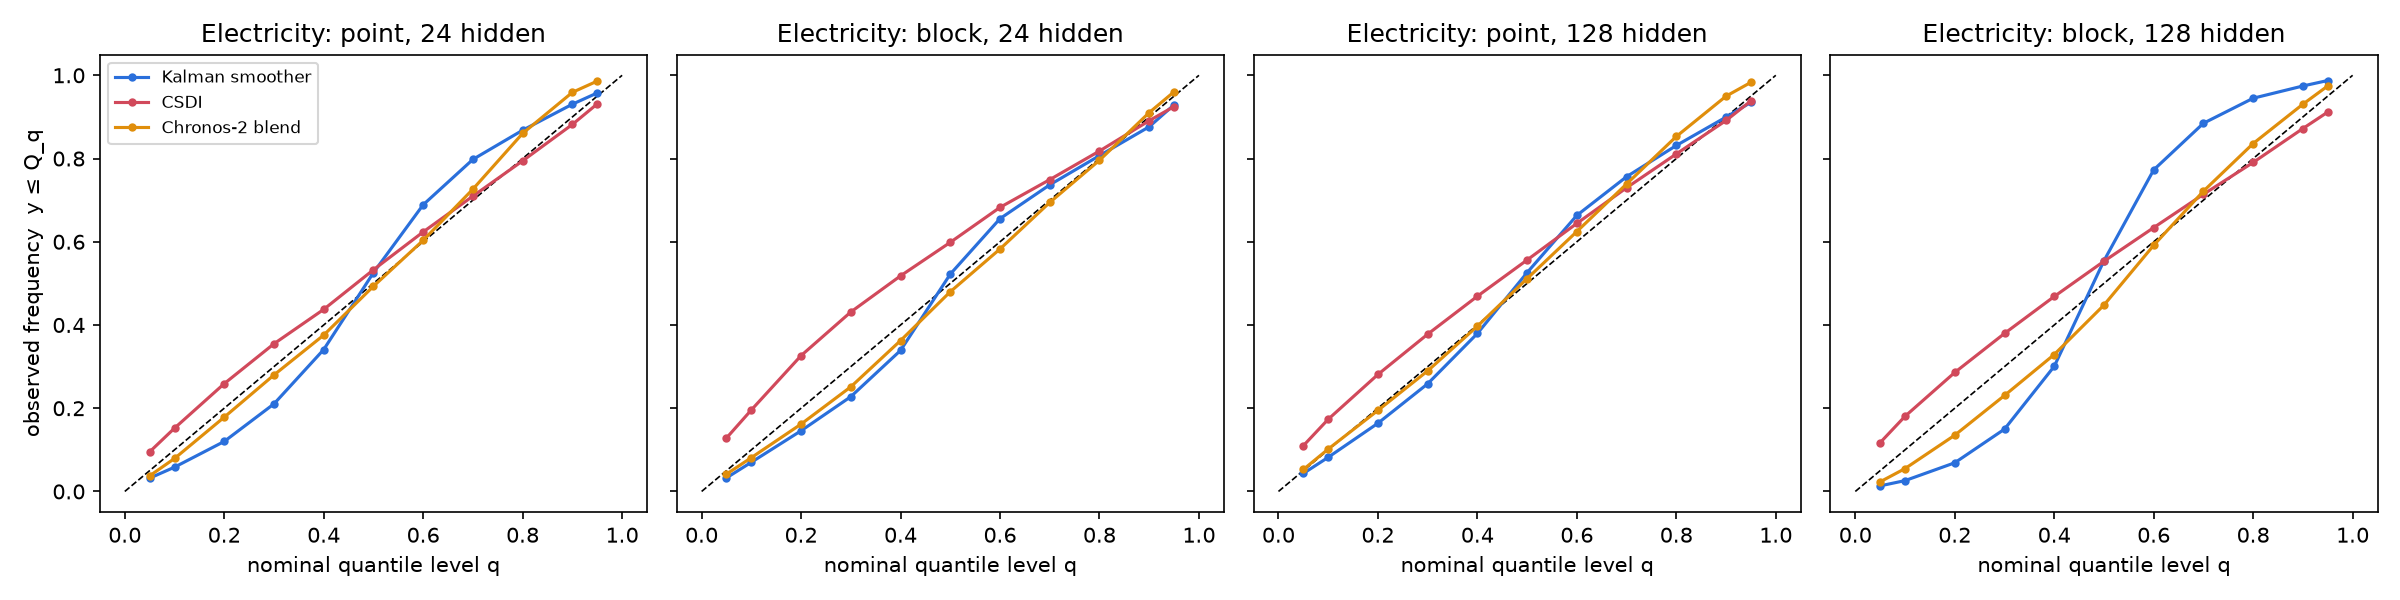
\includegraphics[width=\textwidth]{figures/reliability_test_Electricity.png}
\caption{Reliability on Electricity (test), main run. The curve ``CSDI'' is CSDI-40. Points on the diagonal mean that $y\le Q(\tau)$ occurs with frequency $\tau$. CSDI-40 lies above the diagonal at low $\tau$ and below it at high $\tau$, which means both tails are too thin. Kalman crosses the diagonal steeply on block 128, which means intervals that are too wide.}
\label{fig:reliability}
\end{figure*}

\subsection{Blending the two sides}\label{sec:blend}
The blend improves on one-sided forecasts in 11 of 12 cells (one tie) against both the left-only and the right-only forecast (Table~\ref{tab:pairs}). Mean pinball falls from 0.158 to 0.130. Its coverage rises from 0.775 to 0.831 while the intervals get narrower (width 1.21 to 1.11). Mean PCE is slightly worse (0.025 to 0.034), because CCE changes sign: the one-sided forecasts undercover (CCE $+0.015$) and the blend overcovers ($-0.033$). So the blend moves calibration, and not in a fixed direction (H3).

\textbf{How much too wide?} The blend takes the same kind of average at every quantile level, which gives a wider distribution than the exact conditional one. On a Gaussian random walk with noiseless endpoints and a 24-step gap, the exact standard deviation is $\sigma\sqrt{j(k+1-j)/(k+1)}$. The blend with exact one-sided forecasts is 1.18 times this at the ends and 1.41 times at the midpoint (Figure~\ref{fig:bridge}). The synthetic oracle test measures the same effect with noisy local-level data and the actual \Chr{} forecasts (Table~\ref{tab:variants}, Figure~\ref{fig:oracle}). The linear blend has 80\% intervals 1.11 to 1.24 times the exact width and covers 0.78 to 0.85 (exact: 0.79 to 0.80). Equal weights give 1.34 to 1.50 times and are worse than linear on pinball in all 12 real-data cells. The Gaussian product is too narrow: 0.72 to 0.87 times the exact width, coverage 0.56 to 0.67. On real data PoE covers between 0.51 and 0.80, and linear weights beat it on pinball in 9 of 12 cells.

\begin{table*}[t]
\centering\small
\setlength{\tabcolsep}{5pt}
\begin{tabular}{@{}l ccc cc cc@{}}
\toprule
 & \multicolumn{3}{c}{Real data, 12 cells} & \multicolumn{2}{c}{Synthetic, gap 24} & \multicolumn{2}{c}{Synthetic, gap 128}\\
\cmidrule(lr){2-4}\cmidrule(lr){5-6}\cmidrule(l){7-8}
Forecast & Pinball & Cov.\ 80\% & Width & Width/exact & Cov.\ 80\% & Width/exact & Cov.\ 80\%\\
\midrule
Left only & 0.1579 & 0.775 & 1.211 & 1.36--1.50 & 0.69--0.70 & 1.34--1.37 & 0.61--0.65 \\
Right only & 0.1574 & 0.777 & 1.190 & 1.39--1.51 & 0.69--0.71 & 1.35--1.38 & 0.63--0.64 \\
Linear quantile blend & 0.1298 & 0.831 & 1.115 & 1.19--1.24 & 0.82--0.85 & 1.11--1.13 & 0.78--0.79 \\
Equal-weight blend & 0.1357 & 0.839 & 1.200 & 1.37--1.50 & 0.81--0.84 & 1.34--1.38 & 0.75--0.77 \\
Gaussian product & 0.1361 & 0.699 & 0.726 & 0.85--0.87 & 0.65--0.67 & 0.72--0.74 & 0.56--0.57 \\
\bottomrule

\end{tabular}
\caption{Blend variants. Real data: mean over the 12 test cells. Synthetic: range over the three noise ratios $r/q$; the exact smoother has coverage 0.79--0.80 and width ratio 1.}
\label{tab:variants}
\end{table*}

\begin{figure}[t]
\centering
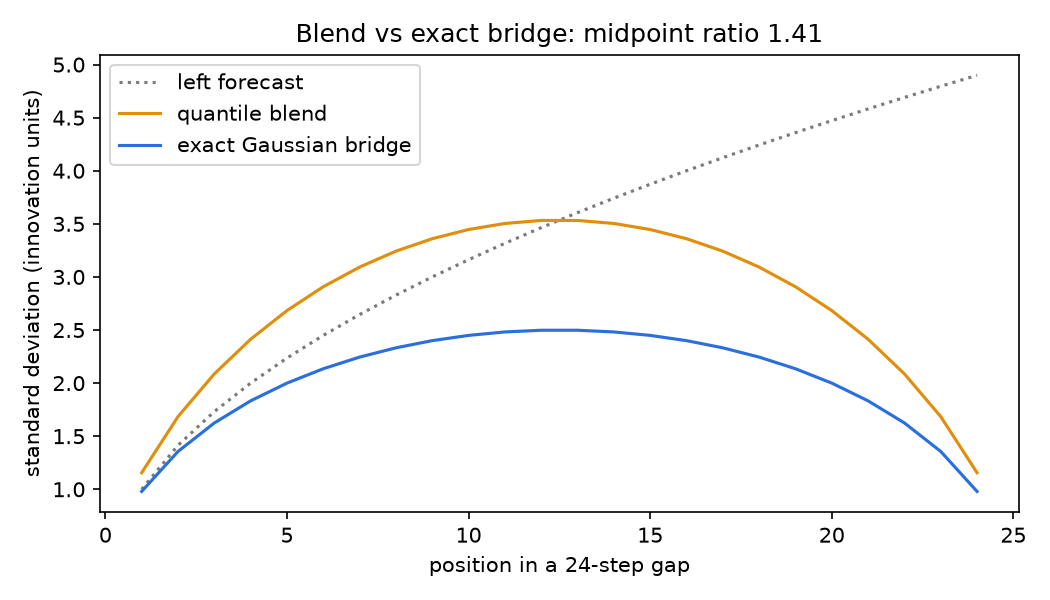
\includegraphics[width=\columnwidth]{figures/bridge.png}
\caption{Standard deviation of the exact Gaussian bridge and of the linear quantile blend of two exact one-sided forecasts (random walk, 24-step gap). The ratio at the midpoint is 1.41.}
\label{fig:bridge}
\end{figure}

\begin{figure*}[t]
\centering
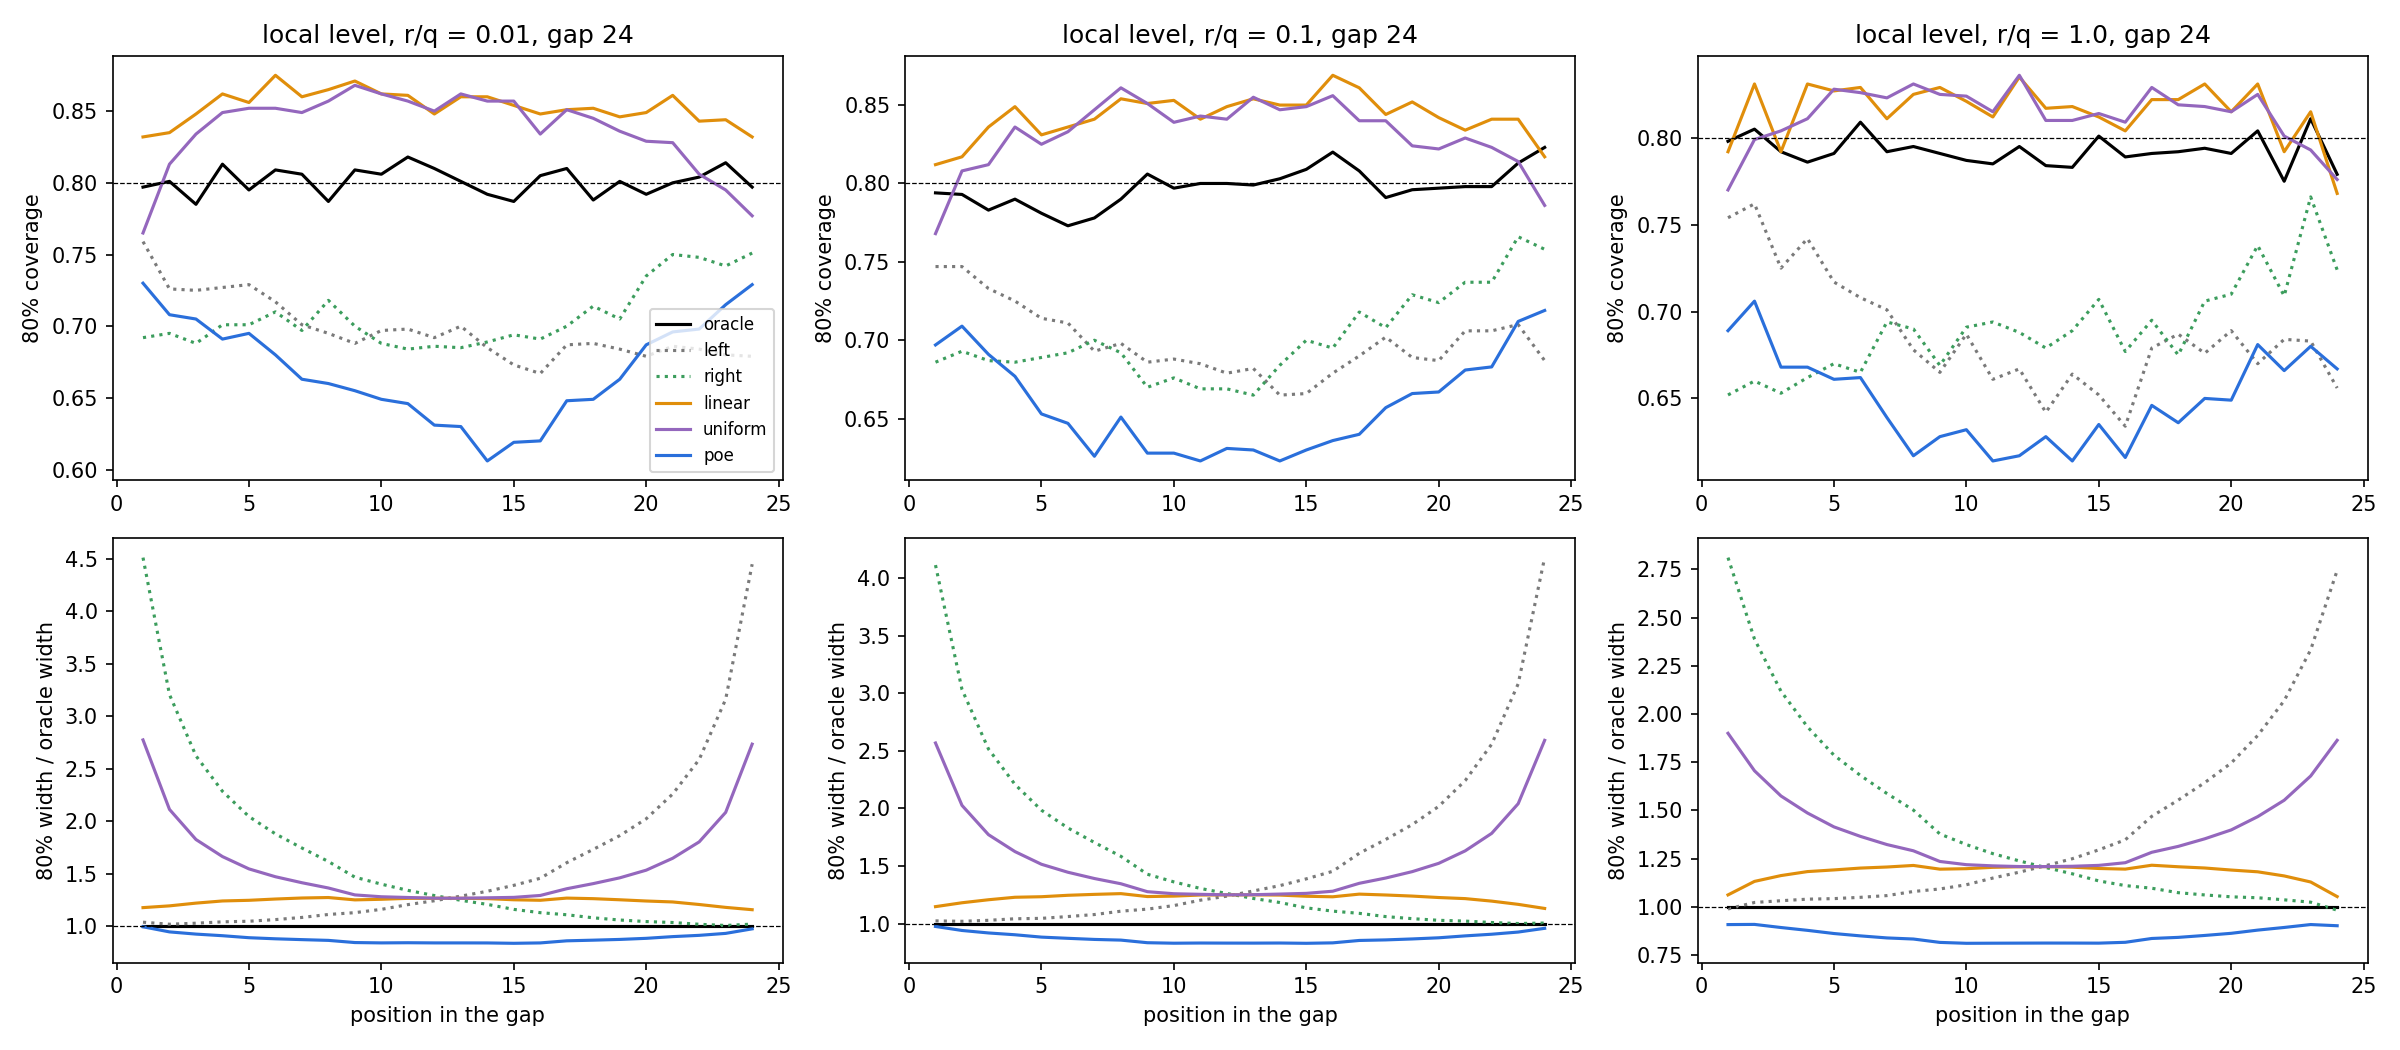
\includegraphics[width=0.92\textwidth]{figures/extra_synthetic_oracle_gap24.png}
\caption{Synthetic oracle test, gap 24. Top: 80\% coverage by position in the gap. Bottom: width relative to the exact smoother. One-sided forecasts are miscentered far from their side. The linear blend is wider than exact (about 1.2 times) and slightly overcovers. The Gaussian product is narrower than exact and undercovers. The gap-128 figure is in the appendix.}
\label{fig:oracle}
\end{figure*}

The one-sided forecasts are on average wider than the exact bridge (1.34 to 1.51 times) and still undercover (0.61 to 0.71). Far from their own side they are centered on the wrong place. A product of two such forecasts is narrow without being correct, which explains the PoE result. We tested PoE in one implementation, with scale taken from three quantiles; a better-fitted variance might do better.

\subsection{Time reversal}\label{sec:reversal}
Chronos-2 forecasts forward. Using it from the right means applying it to the reversed series, which is valid when the process looks the same in both directions. Table~\ref{tab:reversal} tests this on synthetic data. For the reversible AR(1) process the left and right forecasts differ by less than their interval (matched pinball difference $-0.007$ and $+0.006$ for gaps 24 and 128). For the jump process the right forecast is worse on MAE and pinball and covers less: matched pinball differs by $-0.088$ and $-0.112$, and 80\% coverage drops to 0.59 and 0.66 against 0.70 and 0.72. So the test can detect an asymmetry of this size.

On real data (Table~\ref{tab:reversal-real}) the comparison with equal context lengths excludes zero in one of six cases (Electricity gap 24, left better), and the full-context comparison excludes zero in one other case (BeijingAir gap 24, right better). We see no consistent direction. This supports the equal-weight treatment of both sides inside the blend, within the power of the data: with 7 to 19 channels the intervals for pinball are about $\pm0.03$ to $\pm0.09$ wide, and differences of 0.01 to 0.02 stay undetected.

\begin{table*}[t]
\centering\small
\setlength{\tabcolsep}{4.5pt}
\begin{tabular}{@{}llcccccccc@{}}
\toprule
Process & Gap & Context & Len.\ L/R & Pinball L & Pinball R & L$-$R [95\% interval] & Cov.\ L & Cov.\ R\\
\midrule
AR(1), $\phi=0.9$ (reversible) & 24 & full & 116/116 & 0.331 & 0.339 & $-$0.008 [$-$0.020, +0.005] & 0.75 & 0.74 \\
 & 24 & matched & 72/72 & 0.338 & 0.345 & $-$0.007 [$-$0.019, +0.006] & 0.73 & 0.73 \\
 & 128 & full & 64/64 & 0.408 & 0.411 & $-$0.002 [$-$0.014, +0.010] & 0.83 & 0.83 \\
 & 128 & matched & 44/44 & 0.419 & 0.413 & +0.006 [$-$0.007, +0.019] & 0.83 & 0.83 \\
\midrule
Jump process (irreversible) & 24 & full & 118/114 & 0.217 & 0.273 & $-$0.057 [$-$0.092, $-$0.026] & 0.70 & 0.62 \\
 & 24 & matched & 69/69 & 0.221 & 0.309 & $-$0.088 [$-$0.125, $-$0.053] & 0.70 & 0.59 \\
 & 128 & full & 64/64 & 0.269 & 0.351 & $-$0.082 [$-$0.102, $-$0.062] & 0.72 & 0.67 \\
 & 128 & matched & 44/44 & 0.271 & 0.384 & $-$0.112 [$-$0.137, $-$0.087] & 0.72 & 0.66 \\
\bottomrule

\end{tabular}
\caption{Time-reversal test on synthetic data (1,000 windows per row). L: forecast from the left side, R: forecast from the reversed right side. ``Full'' uses all available context, ``matched'' uses the same context length and horizon on both sides.}
\label{tab:reversal}
\end{table*}

\begin{table}[t]
\centering\small
\footnotesize\setlength{\tabcolsep}{2.5pt}
\begin{tabular}{@{}lcll@{}}
\toprule
Dataset & Gap & Full context & Matched context\\
\midrule
ETT\_h1 & 24 & +0.005 [$-$0.024, +0.042] & +0.004 [$-$0.024, +0.039] \\
 & 128 & $-$0.008 [$-$0.049, +0.027] & $-$0.006 [$-$0.040, +0.027] \\
Electricity & 24 & $-$0.035 [$-$0.085, +0.001] & $-$0.041 [$-$0.087, $-$0.009]$^*$ \\
 & 128 & +0.011 [$-$0.021, +0.052] & +0.008 [$-$0.011, +0.035] \\
BeijingAir & 24 & +0.058 [+0.002, +0.115]$^*$ & +0.051 [$-$0.023, +0.114] \\
 & 128 & $-$0.035 [$-$0.091, +0.033] & $-$0.025 [$-$0.103, +0.069] \\
\bottomrule

\end{tabular}
\caption{Real data: pinball of the left forecast minus the right forecast, with 95\% bootstrap interval. $^*$: interval excludes zero.}
\label{tab:reversal-real}
\end{table}

\subsection{Training budget of CSDI}\label{sec:budget}
Table~\ref{tab:budget} compares the two schedules. Validation loss is 8.3\% to 13.4\% lower with CSDI-100, mean test pinball falls by 18\% on average, and it improves in every cell of every dataset (12 of 12 on mean pinball; the paired test gives 11 wins and one tie). The best epochs of CSDI-100 are 92 to 97 of 100, and the loss curves are still sloping down slightly at the end (Figure~\ref{fig:curves}). One more doubling of the budget might still help; we did not run it. CSDI-40 on Electricity hit the 40-epoch cap, so early stopping did not apply there. On ETT\_h1 and BeijingAir early stopping ended CSDI-40 at epochs 31 and 35, and the longer schedule still lowered their validation loss by 13.4\% and 8.3\%. Early stopping did not show that these two runs had converged.

\begin{table*}[t]
\centering\small
\setlength{\tabcolsep}{5pt}
\begin{tabular}{@{}lcccccccc@{}}
\toprule
 & \multicolumn{2}{c}{CSDI-40} & \multicolumn{2}{c}{CSDI-100} & & \multicolumn{2}{c}{Test pinball, mean of 4 cells} & Cells\\
\cmidrule(lr){2-3}\cmidrule(lr){4-5}\cmidrule(lr){7-8}
Dataset & Epochs / best & Val.\ loss & Epochs / best & Val.\ loss & Gain & CSDI-40 & CSDI-100 & improved\\
\midrule
ETT\_h1 & 31 / 26 & 0.1966 & 100 / 97 & 0.1702 & 13.4\% & 0.1548 & 0.1139 & 4/4 \\
Electricity & 40 / 39 & 0.2117 & 100 / 92 & 0.1877 & 11.3\% & 0.1045 & 0.0917 & 4/4 \\
BeijingAir & 35 / 30 & 0.1454 & 100 / 94 & 0.1334 & 8.3\% & 0.1571 & 0.1356 & 4/4 \\
\bottomrule

\end{tabular}
\caption{Training budget. ``Val.\ loss'' is the best masked validation loss. Gain is the relative fall in validation loss.}
\label{tab:budget}
\end{table*}

\begin{figure*}[t]
\centering
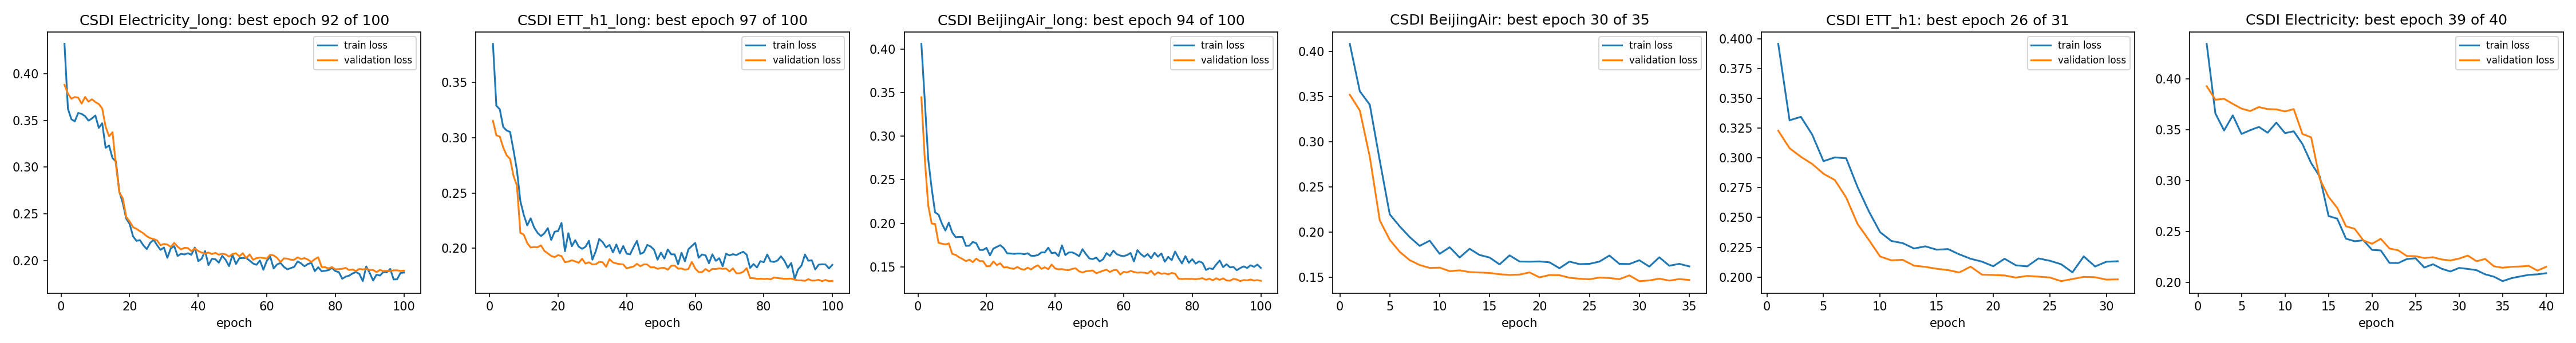
\includegraphics[width=\textwidth]{figures/extra_csdi_curves.png}
\caption{Training and validation loss. Left three: CSDI-100 (Electricity, ETT\_h1, BeijingAir). Right three: CSDI-40. The 40-epoch runs stop where the constant-rate loss flattens; the 100-epoch runs continue after each learning-rate drop.}
\label{fig:curves}
\end{figure*}

\subsection{Sensitivity of the ranking to the CRPS estimate}
Our first CRPS columns use three estimates that differ across model families. Among Kalman, CSDI-40 and the blend, the winner by pinball differs from the winner by these CRPS values in 2 of 12 cells (BeijingAir block 24, Electricity point 24). With CRPS$_{21}$, the same 21-level approximation for all models, the winners agree with pinball in all 12 cells, and also when CSDI-100 is added. We therefore use pinball on nine levels as the common score and read CRPS values only inside one family or as CRPS$_{21}$.

\section{Discussion, Limitations and Negative Results}\label{sec:limits}
\textbf{What the results say.} No imputer in this study returns reliable 80\% intervals across all cells. CSDI errs toward intervals that are too narrow, Kalman and the blend toward intervals that are too wide in most cells, and each fails somewhere else: Kalman is far off on long blocks, the blend on long BeijingAir gaps, CSDI nearly everywhere by a similar amount. Accuracy and calibration do not rank the models the same way (H2). The blend is a cheap way to get a two-sided imputer from a forecaster, it is better than the one-sided forecasts, and it is wider than exact inference by a measurable factor. CSDI-100 is more accurate than the blend and has a lower PCE on average (0.027 against 0.034), but its CCE is larger in absolute value (0.047 against $-0.033$), it needs training per dataset, and it still undercovers.

\textbf{Negative results.}
\begin{itemize}
\item Training CSDI for 100 epochs did not fix undercoverage: CCE stays positive in all 12 cells.
\item The Gaussian product of the two forecasts was worse than the linear blend (9 of 12 cells on pinball) and badly undercovers. Equal-weight blending lost to linear weights in all 12 cells.
\item On real data the time-reversal test found no consistent effect. The synthetic jump process shows that the question matters in principle, but we cannot say whether a real dataset here has such an asymmetry.
\item A first long CSDI run failed. PyPOTS steps the learning-rate scheduler after every batch, and we had set the milestones in epochs, so the rate fell to $10^{-5}$ inside the first epoch and the validation loss stayed near 0.37. We discarded the run and set the milestones in steps (14,100 and 16,920). The log of the failed run is kept in the repository.
\item The CSDI-40 results that the poster and the main tables (\texttt{metrics\_*.csv}) still show were under-trained, and the conclusions drawn from them were weaker than the CSDI-100 results allow.
\end{itemize}

\textbf{Deviations from the plan.} The project charter did not plan significance statements. The paired cluster bootstrap, the synthetic tests, the CRPS$_{21}$ grid and the long CSDI run were added after the peer review. The CSDI-100 recipe was not tuned: it was fixed once and run once per dataset, with validation loss only picking the epoch. It was chosen after we had seen the CSDI-40 test results, which is the order of events a reader should keep in mind.

\textbf{Fairness of the comparison.} CSDI-100 receives much more optimization than the baselines: Kalman fits two numbers per channel, and \Chr{} is frozen and used with default settings. We did not tune any model on the test split. CSDI is univariate and cannot use other channels, and the Kalman smoother has no seasonality; a seasonal state-space model would be a stronger classical baseline, and we did not build one.

\textbf{Limitations.}
\begin{itemize}
\item CSDI-100 uses one seed and 100 epochs; the best epochs (92 to 97) are near the end of training. Seed variation is unmeasured.
\item Masks are synthetic and drawn from windows without native missing values. The count of eligible windows per dataset was not recorded.
\item Channels and windows are dependent, and the bootstrap rests on 7 to 19 channels. We did not correct for multiple comparisons, so single verdicts are indications only.
\item Synthetic tests cover a local-level process and two control processes. They have no seasonality. PoE was tested in one implementation.
\item The main run was on an Apple M4 (MPS) and the CSDI-100 runs on a Colab T4 (CUDA). Samples and results of the two setups are not bit-identical.
\item \Chr{} pretraining overlap with our datasets was not checked.
\item Finite diffusion samples (100 draws) limit the accuracy of CSDI tail quantiles.
\end{itemize}

\section{Reproducibility and Compute}
\textbf{Code and revision.} The code, configurations and saved predictions are in the repository at revision \revision. Data are downloaded with \texttt{tsdb} and prepared by \texttt{python -m tsi.data --config configs/main.yaml}. The main experiment runs with \texttt{./run\_all.sh}. The additional analyses (CSDI-100, blend variants, synthetic tests, bootstrap) run in the order of \texttt{colab\_extra.ipynb}. Every table of this paper is produced by \texttt{paper/make\_tables.py} from the CSV files in \texttt{results/tables/}, and the figures are produced by the evaluation scripts. The numbers in the paper, the README and the presentation come from the same files.

\textbf{Seeds and configurations.} Windows and masks use fixed NumPy seeds (validation 1, test 2, train 0). The CSDI-40 run did not set the PyTorch seed, so a new fit will not match it exactly; its outputs are saved. CSDI-100 sets \texttt{torch.manual\_seed(0)} and the CUDA seed. Settings are in \texttt{configs/main.yaml} (shared), \texttt{configs/long.yaml} and \texttt{configs/long2.yaml} (CSDI-100; Electricity, and ETT\_h1 with BeijingAir). Python dependencies are in \texttt{requirements.txt}.

\textbf{Compute.} Main run on an Apple M4 with 24 GB: CSDI-40 training took 0.35 h (ETT\_h1), 0.54 h (Electricity) and 0.37 h (BeijingAir); the first two are reconstructed from log timestamps, and BeijingAir test sampling took about 0.58 h. \Chr{} ran on the CPU. The CSDI-100 runs and the additional analyses ran on one NVIDIA T4 in Google Colab: 0.30 h of training per dataset and 0.10 h of sampling per split and dataset. Times from the two machines are not comparable.

\section{Contributions and Use of AI}
\textbf{Author contributions.}
\begin{itemize}
\item Vladislav Voronin: additional model training.
\item Kirill Lalayants: data collection, initial model training.
\item Mikhail Bezrukov: initial model training.
\item Fedor Zhirkov: choosing metrics, verifying data and cross-checking results.
\end{itemize}

\textbf{Use of AI assistance.} Consulting and assistance in making paper review.

\section*{Acknowledgements}
We thank our supervisor Vitaliy Pozdnyakov and the peer reviewers for comments that led to the CSDI-100 run and to the synthetic tests.

{\small
\bibliographystyle{plainnat}
\bibliography{references}
}

\clearpage
\onecolumn
\appendix
\section{Appendix}
\subsection{Calibration in every cell}
\begin{table}[htbp]
\centering\footnotesize
\setlength{\tabcolsep}{3.2pt}
\begin{tabular}{@{}l cccc cccc cccc@{}}
\toprule
 & \multicolumn{4}{c}{Coverage of 80\% intervals} & \multicolumn{4}{c}{PCE} & \multicolumn{4}{c}{Width of 80\% intervals}\\
\cmidrule(lr){2-5}\cmidrule(lr){6-9}\cmidrule(l){10-13}
Cell & Kal. & C-40 & Blend & C-100 & Kal. & C-40 & Blend & C-100 & Kal. & C-40 & Blend & C-100\\
\midrule
ETT\_h1 point 24 & 0.833 & 0.751 & 0.847 & 0.739 & 0.039 & 0.047 & 0.024 & 0.021 & 0.70 & 0.63 & 0.78 & 0.52 \\
ETT\_h1 block 24 & 0.707 & 0.702 & 0.787 & 0.749 & 0.063 & 0.071 & 0.039 & 0.037 & 1.79 & 1.04 & 1.05 & 0.98 \\
ETT\_h1 point 128 & 0.793 & 0.730 & 0.842 & 0.745 & 0.020 & 0.072 & 0.019 & 0.019 & 0.90 & 0.78 & 1.02 & 0.64 \\
ETT\_h1 block 128 & 0.917 & 0.675 & 0.863 & 0.750 & 0.074 & 0.133 & 0.032 & 0.016 & 3.91 & 1.37 & 1.68 & 1.13 \\
\midrule
Electricity point 24 & 0.872 & 0.730 & 0.880 & 0.736 & 0.055 & 0.032 & 0.026 & 0.024 & 0.82 & 0.52 & 0.73 & 0.43 \\
Electricity block 24 & 0.806 & 0.695 & 0.829 & 0.714 & 0.036 & 0.076 & 0.020 & 0.038 & 2.19 & 0.72 & 0.93 & 0.66 \\
Electricity point 128 & 0.818 & 0.718 & 0.848 & 0.732 & 0.029 & 0.048 & 0.021 & 0.025 & 1.09 & 0.62 & 0.96 & 0.53 \\
Electricity block 128 & 0.948 & 0.692 & 0.876 & 0.722 & 0.105 & 0.051 & 0.041 & 0.026 & 4.82 & 0.84 & 1.56 & 0.81 \\
\midrule
BeijingAir point 24 & 0.928 & 0.765 & 0.903 & 0.746 & 0.099 & 0.030 & 0.059 & 0.016 & 0.50 & 0.33 & 0.60 & 0.29 \\
BeijingAir block 24 & 0.835 & 0.660 & 0.785 & 0.710 & 0.042 & 0.069 & 0.015 & 0.033 & 1.38 & 1.33 & 1.36 & 1.15 \\
BeijingAir point 128 & 0.905 & 0.734 & 0.848 & 0.738 & 0.084 & 0.029 & 0.065 & 0.027 & 0.67 & 0.46 & 0.81 & 0.42 \\
BeijingAir block 128 & 0.841 & 0.598 & 0.670 & 0.717 & 0.040 & 0.109 & 0.051 & 0.038 & 3.05 & 1.88 & 1.90 & 1.93 \\
\bottomrule

\end{tabular}
\caption{Test coverage, PCE and width per cell. Kal.: Kalman; C-40: CSDI-40; Blend: \Chr{} blend; C-100: CSDI-100. Width is in train-scaled units.}
\label{tab:calib}
\end{table}

\subsection{Further figures}
\begin{figure}[htbp]
\centering
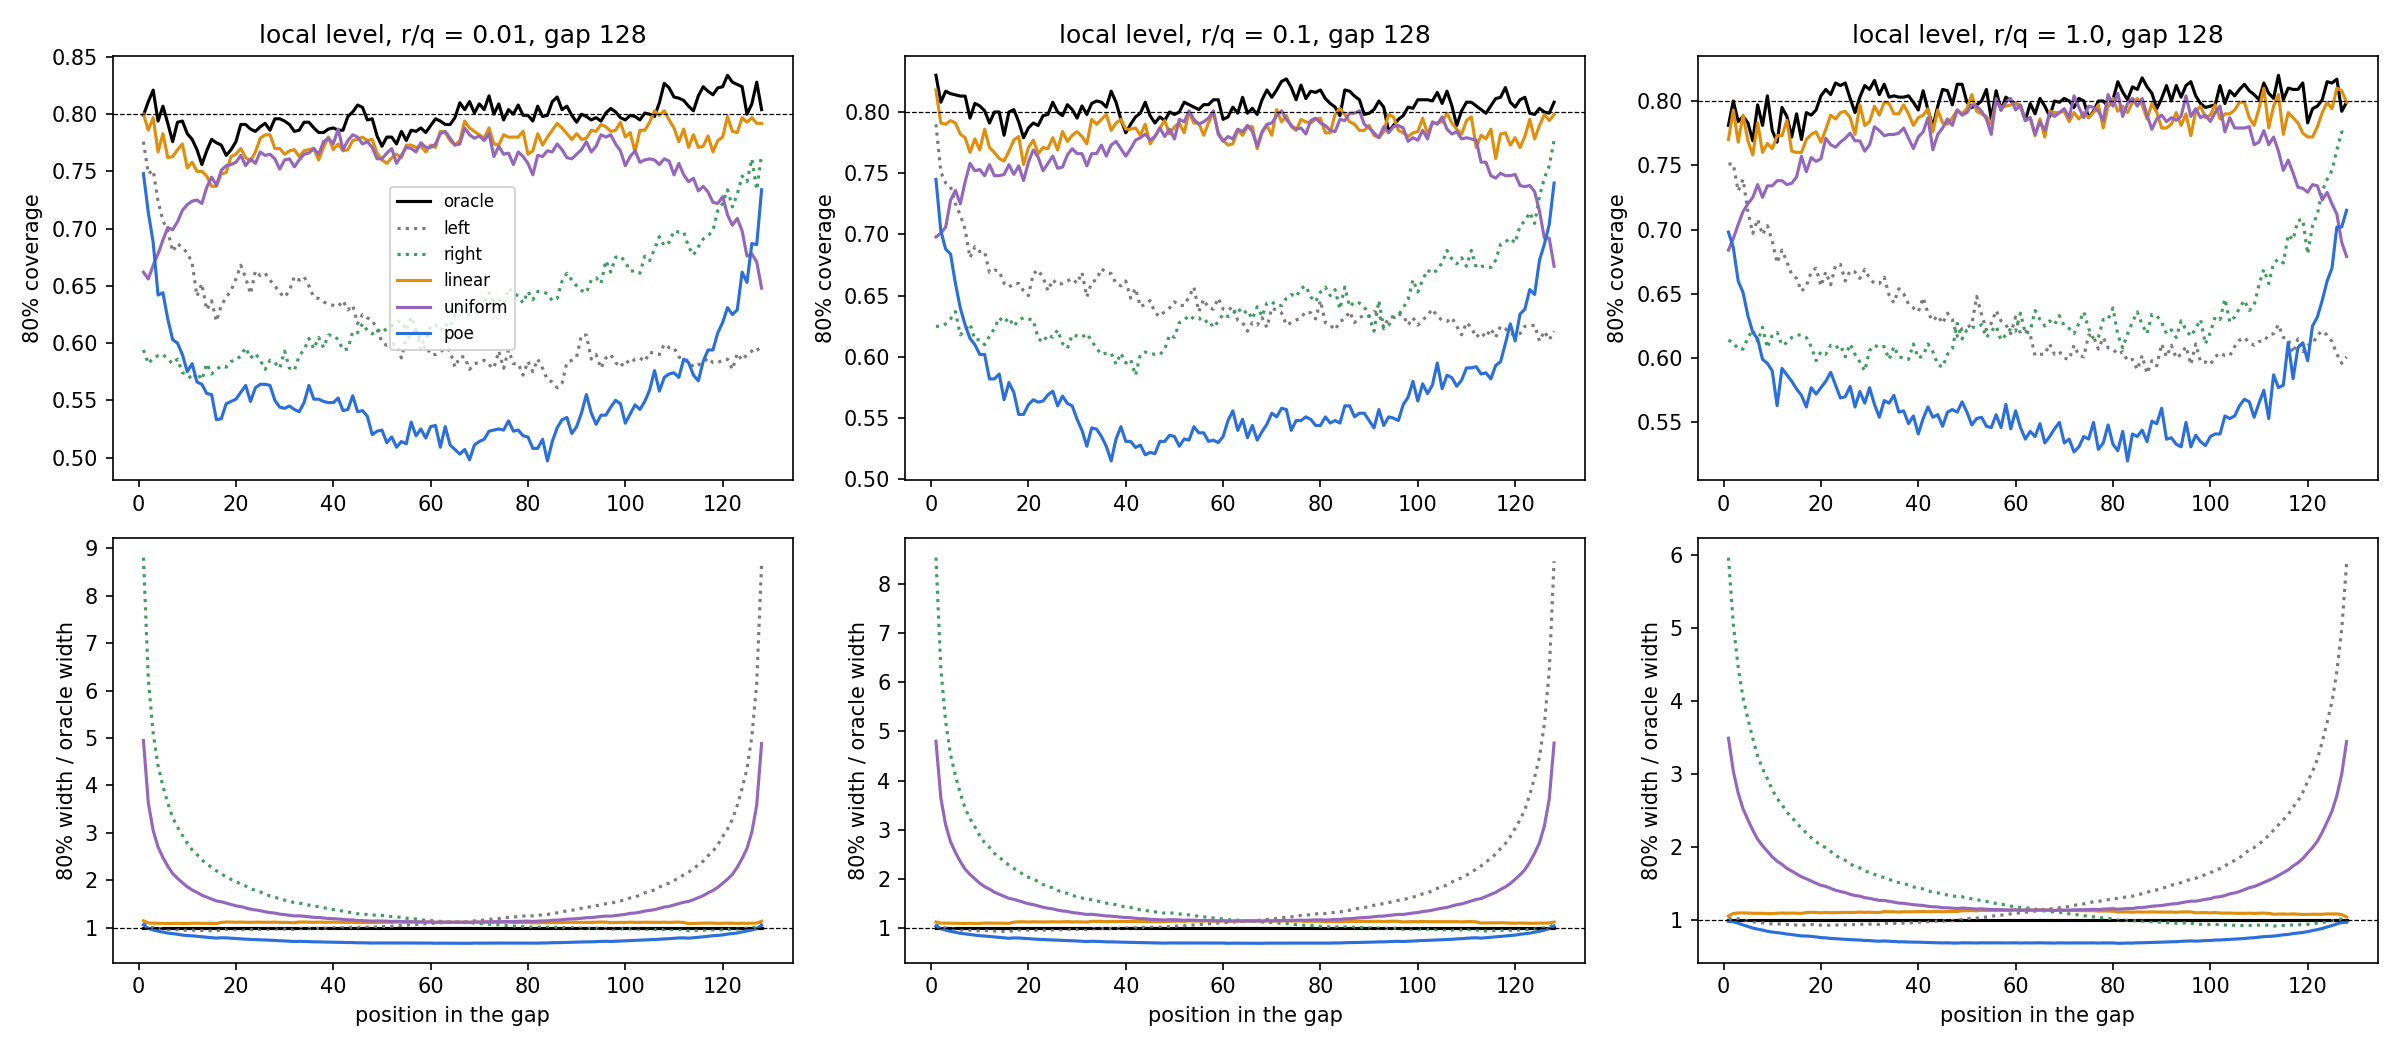
\includegraphics[width=0.85\textwidth]{figures/extra_synthetic_oracle_gap128.png}
\caption{Synthetic oracle test, gap 128 (same layout as Figure~\ref{fig:oracle}).}
\end{figure}
\begin{figure}[htbp]
\centering
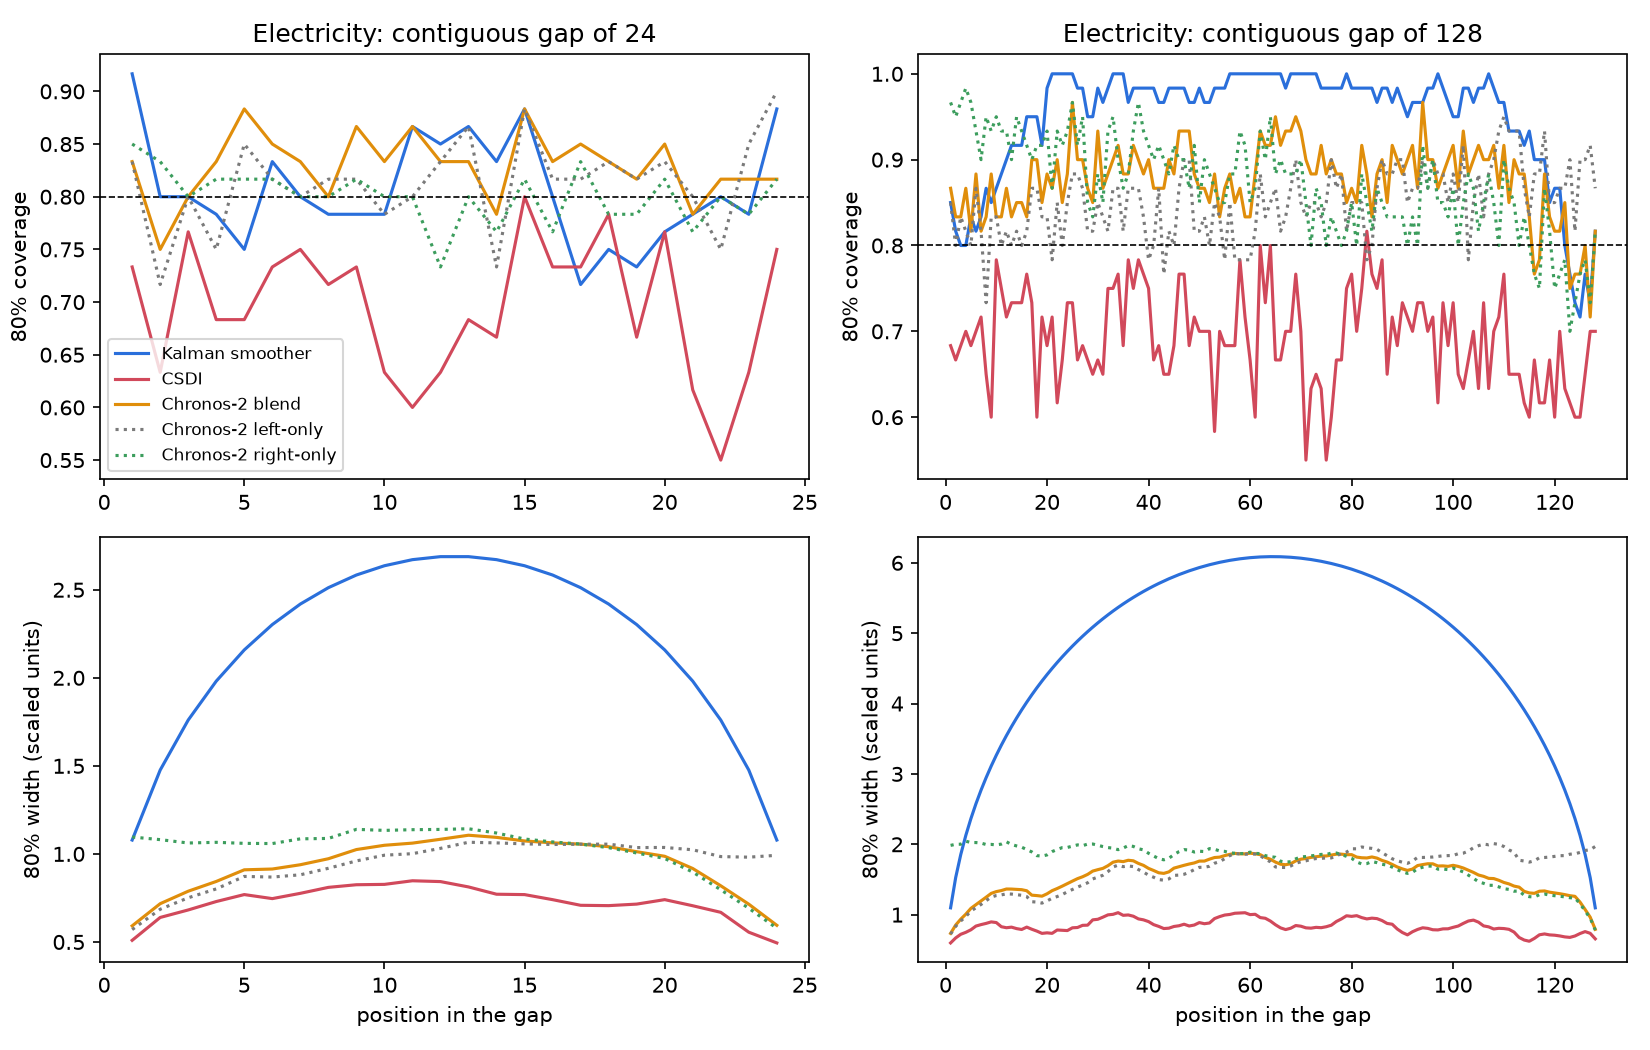
\includegraphics[width=0.7\textwidth]{figures/along_gap_test_Electricity.png}
\caption{Electricity test, block gaps of 24 and 128: 80\% coverage and width by position in the gap, main run (``CSDI'' is CSDI-40). The Kalman width is an arc that grows with the distance from the edges; CSDI intervals stay narrow and flat, and the blend narrows near the edges.}\label{fig:along}
\end{figure}

\subsection{Configuration summary}
Windows of 256 steps, edge 24, hidden counts 24 and 128, patterns point and block, 60 windows per dataset and split, quantile levels $0.05,0.1,\dots,0.9,0.95$ (11 levels saved in the main run; 21 levels for CRPS$_{21}$). CSDI: 4 layers, 8 heads, 64 channels, time embedding 128, feature embedding 16, diffusion embedding 128, 50 diffusion steps, 100 samples, sampling batch of 400 rows. Kalman: variances fitted on the last 6,000 train points. \Chr{}: \texttt{autogluon/chronos-2-small}, CPU, batch size 256.

\end{document}
